\documentclass{beamer}

\usepackage{amssymb,amsmath,amsfonts,amsthm}
\usepackage{mathrsfs}
\usepackage{verbatim}
\usepackage{hyperref}

\title{Getting Lean up and Running}
\author{Matej Penciak}
\institute{Northeastern University}
\date{February 11, 2022 \\ Slides available at: \\ \url{https://github.com/mpenciak/Lean-Seminar-Sp2022}}

\begin{document}

% Title Slide
\frame{\titlepage}

\begin{frame}
    \frametitle{A good tweet}
    \begin{center}
        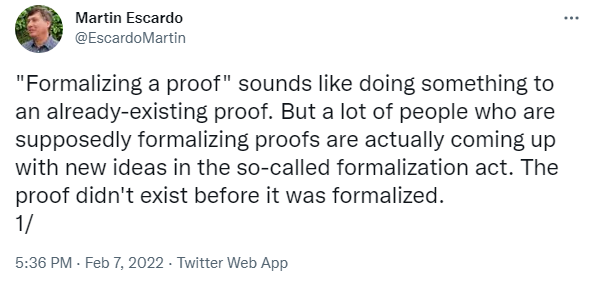
\includegraphics[scale=.6]{img/martin_tweet.png}
    \end{center}
    \url{https://twitter.com/EscardoMartin/status/1490816890414972930}

\end{frame}

\begin{frame}
    \frametitle{Parts of the toolchain}
    \begin{enumerate}
        \setcounter{enumi}{-1}
        \item Bash (or any other shell)
        \item Lean 3
        \begin{itemize}
            \item lean
            \item elan
            \item leanpkg
        \end{itemize}
        \item Git
        \item Python 3
        \begin{itemize}
            \item mathlibtools
        \end{itemize}
        \item VS Code or emacs
        \begin{itemize}
            \item Including the lean extension
        \end{itemize}
    \end{enumerate}
\end{frame}

\begin{frame}
    \frametitle{Shell}

    This should only matter if you're on Windows. There are a number of options to get a Unix-like shell on Windows (msys2, cygwin) but the recommended way is to get the git bash client from \url{https://gitforwindows.org/}

    (this has the added benefit of dealing with step 2 as well).
    \vspace{10pt}

    If you're feeling fancy pretty much everything below works with other shells as well (zsh, fish, ...) with maybe slight modifications to add things to your path variable when the time comes.
    

\end{frame}
\begin{frame}
    \frametitle{Lean}

    Lean is distributed with handy install scripts most platforms. Just follow the instructions for your particular setup at \url{https://leanprover-community.github.io/get_started.html}. They should all be fairly painless (except maybe on new Macs with M1 chips)
    \vspace{10pt}

    What was installed:
    \begin{itemize}
        \item lean (Lean 3): This is the essence of Lean. It includes the interpreter
        \item elan: (Kind of like venv for Python or cabal for Haskell)
        \item leanpkg: A built-in
    \end{itemize}

\end{frame}

\begin{frame}
    \frametitle{Git}

    Git (for those of you who are unaware) is a handy program that creates repositories and can handle version control of said repos. 
    \vspace{10pt}

    Windows: Hopefully you got it along with Git Bash above. 
    \vspace{10pt}

    Linux: Most (all?) distros should already have it installed. If not just use your package manager.
    \vspace{10pt}

    OSX: A few options are available to install it. Probably the easiest is to get the installer binary \url{https://sourceforge.net/projects/git-osx-installer/}.
    \vspace{10pt}
\end{frame}

\begin{frame}[fragile]
    \frametitle{Python}

    Again, all Linux distributions and OSX come with Python pre-installed so this only affects Windows users.On Windows just install the latest version of Python at \url{https://www.python.org/}.
    \vspace{10pt}

    It may seem strange that we need Python in order to work with Lean, and to a certain extent this is true and will change with Lean 4.
    \vspace{10pt}
    
    Until then you will need a python utility called leanproject. Get it with \verb!python -m pip install mathlibtools!. 


\end{frame}

\begin{frame}
    \frametitle{VS Code}

    Lean has a limited list of editors that support interactive theorem proving. This list includes VS Code and emacs (and unofficially neovim \url{https://github.com/Julian/lean.nvim/}).
    \vspace{10pt}
    
    The easiest to get up and running is VS Code ({\bf Opinion:} Which all of you should be using anyway) \url{https://code.visualstudio.com/}

    (for non debian Linux distros, use your package manager)
    \vspace{10pt} 

    You will also need the Lean extension. Don't get lean4 (version v0.0.63), get lean (version v0.16.45). 

\end{frame}

\begin{frame}[fragile]
    \frametitle{Lean Projects}

    If everything is working correctly you should be able to run 
    \begin{verbatim}
    leanproject get
    https://github.com/mpenciak/Lean-Seminar-Sp2022.git
    \end{verbatim}
    and download these slides, all the demos, and everything that comes after that.
    \vspace{10pt}

    \verb!leanproject! is an amalgamation scripts that run leanpkg to set up the structure of the Lean project and add mathlib as a dependency, and git to get all the dependencies. 
    \vspace{10pt}

    Keep up to date by running \verb!leanproject pull! occasionally. 
\end{frame}

\begin{frame}[fragile]
    \frametitle{Lean Projects structure}
    \begin{enumerate}
        \item \verb!leanpkg.toml! File that keeps track of the package information, dependencies, and more
        \item \verb!leanpkg.path! File that tells leanpkg where to look for dependencies when we type things like \verb!import data.nat.basic!
        \item \verb!.gitignore! File that tells what files/folders git can ignore. 
        \item \verb!./src/! Put all of your .lean files in this folder!
        \item \verb!./_target/! This is where all of the dependencies are installed for the project. Note this is in .gitignore because leanproject knows where to look for them from \verb!leanpkg.toml!
    \end{enumerate}
\end{frame}

\begin{frame}[fragile]
    \frametitle{Lets get to actually using Lean!}

    Either run \verb!leanproject new <name>! to start a new project with mathlib dependencies or \verb!leanproject get <name>! to start working on an ongoing project. 
    \vspace{10pt}

    Everything should be working if when you open \verb!/src/week1/Demo1.lean! your editor doesn't yell at you, and the ``lean infoview'' panel opens automatically. 
\end{frame}

\end{document}